% cv-us.tex
%
% Jason R. Blevins - Curriculum Vitae
%
% Copyright (C) 2004-2005 Jason Blevins <jrb11@duke.edu>
%
%%---------------------------------------------------------------------------
%
% Notes:
%
% * To create a new page use
%   \newpage \opening
%
% * res.cls includes an \address{} command which can be used up to twice,
%   but my address is too long for the format it uses.
%
% * Alternate documentclass command:
%   \documentclass[margin,line,11pt,final]{res}
%
% * When publication/presentation list gets longer, divide into subsections
%   by year like this:
%   \section{\bf\small\hspace{8mm}2005}
%
%%---------------------------------------------------------------------------- 

% some CV tips
% http://www.cvtips.com/
% 

\documentclass[overlapped,line,10pt,letterpaper]{res}
\usepackage{hyperref}
% \usepackage{fullpage}

% compact itemized listings
% http://texdoc.net/texmf-dist/doc/latex/enumitem/enumitem.pdf
\usepackage{enumitem}

% required to place logo
\usepackage{graphicx}
\usepackage{picture}
\usepackage{eso-pic}


\hypersetup{
  colorlinks=true,
  urlcolor=blue,
  pdftitle={Dylan E. Beaudette: Curriculum Vitae},
  pdfauthor={Dylan E. Beaudette},
  pdfcreator={\LaTeX\ with package \flqq hyperref\frqq},
  pdfsubject={Curriculum Vitae},
  pdfkeywords={soil pedology terrain analysis landscape modeling energy budget flux pedogenesis geomorphology}
}


%%===========================================================================%%



\begin{document}

% add logo: note manual placement and sizing
\AddToShipoutPicture*{\put(92,\dimexpr\paperheight-3.05cm){%
  \makebox[\paperwidth]{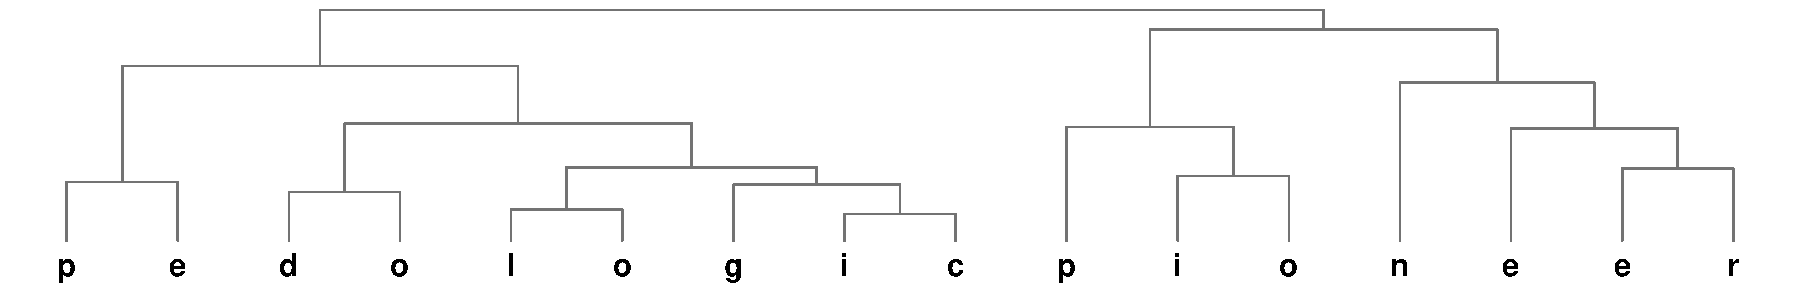
\includegraphics[height=1.33cm]{logo-dend.pdf}}%
}}


\name{Dylan E. Beaudette}

\begin{resume}

\begin{format}
\employer{l}\location{r}\\
\title{l}\dates{r}\\
\end{format}

\begin{ncolumn}{2}
  USDA-NRCS    						& Phone: 209.591.5180\\
  Sonora MLRA Soil Survey Office    & E-mail: dylan.beaudette@usda.gov\\
  19777 Greenley Road				& E-mail: debeaudette@ucdavis.edu\\
  Sonora, CA 95370   USA   			& Web: \small{http://casoilresource.lawr.ucdavis.edu/soilweb}
\end{ncolumn}

%---------------------------------------------------------------------------
\section{\bf Employment}

\employer{USDA-NRCS}
\title{Soil Scientist, Digital Soil Mapping Specialist}
\location{Lincoln, NE, USA}
\dates{2018 -- Current}
\begin{position}
\begin{minipage}{0.95\textwidth}
Soil Business Systems\\
Southwest Regional Soil Data Quality Specialist (detail)
\end{minipage}
\end{position}

\employer{USDA-NRCS}
\title{Soil Scientist, Digital Soil Mapping Specialist}
\location{Davis, CA, USA}
\dates{2017 -- 2018}
\begin{position}
\begin{minipage}{0.95\textwidth}
SSR2 Soil Data Quality Specialist
\end{minipage}
\end{position}

\employer{USDA-NRCS}
\title{Soil Scientist, Digital Soil Mapping Specialist}
\location{Davis, CA, USA}
\dates{2013 -- 2017}
\begin{position}
\begin{minipage}{0.95\textwidth}
SSR2 Staff
\end{minipage}
\end{position}

\employer{Columbia Junior College}
\title{Adjunct Faculty}
\location{Columbia, CA, USA}
\dates{2013 -- 2015}
\begin{position}
\end{position}

\employer{USDA-NRCS}
\title{Soil Scientist}
\location{Sonora, CA, USA}
\dates{2011 -- 2013}
\begin{position}
\end{position}

%---------------------------------------------------------------------------
\section{\bf Education}
Ph.D. Soils \& Biogeochemistry, June 2011 \newline
University of California at Davis, Davis, CA, USA
\\
\begin{minipage}{0.95\textwidth}
\hrule
\begin{itemize}[itemsep=0.05cm,leftmargin=*]
\small
\vspace{0.125cm}

	\item Quantitative partitioning of variance in soil physical and chemical properties across hillslope and lithologic gradients within the Sierra Nevada Foothill Region of California.
	
	\item Quantitative evaluation of commonly used terrain-shape indices for digital soil mapping (via sensor networks) in the Sierra Nevada Foothill Region of California.
	
	\item Extension of the SoilWeb platform to mobile devices.
	
	\item Development of new approaches to numerical classification of soil profiles based on morphologic and laboratory data.
	
	\item Development of paired field--lab devices for measuring mineral weathering rates, supporting simulation of the effects of long-term climate change on soil and ecosystem parameters.
	
\end{itemize}
\vspace{0.125cm}
\hrule
\end{minipage}

M.Sc. Soils \& Biogeochemistry, March 2008 \newline
University of California at Davis, Davis, CA, USA
\\
\begin{minipage}{0.95\textwidth}
\hrule
\begin{itemize}[itemsep=0.05cm,leftmargin=*]
\small
\vspace{0.125cm}
	
	\item Quantification of the ``aspect effect'' via modeled solar radiation data, and applications to soil survey investigations.
	
	\item Development of an online interface to USDA-NCSS digital soil survey products with an emphasis on education and outreach (SoilWeb).
	
	\item Initial soil mapping in Pinnacles National Monument, CA.
	
\end{itemize}
\vspace{0.125cm}
\hrule
\end{minipage}

B.S. Environmental Resource Science (GIS and Remote Sensing emphasis)\newline Minor in Japanese, June 2004 \newline
University of California at Davis, Davis, CA, USA

%---------------------------------------------------------------------------
\section{\bf Contributions to the Academic / Scientific Community}
Regular reviewer for many of the top soil science journals:
\begin{itemize}[itemsep=0.05cm]
	\small
	\item Soil Science Society of America Journal
	\item Geoderma
	\item Soil and Water Conservation
	\item Soil Science
	\item Catena
\end{itemize}

Regular contributor to the open-source software community:
\begin{itemize}[itemsep=0.05cm]
	\small
	\item active development and testing of R packages related to earth sciences
	\item past member of the GRASS GIS project steering committee
	\item contributor to the GRASS GIS codebase, documentation, and mailing list
	\item contributor to the r-help and r-sig-geo mailing lists
	\item contributor to the gdal and postgis mailing lists
\end{itemize}

The \href{http://ncss-tech.github.io/AQP/}{Algorithms for Quantitative Pedology project}: code, tutorials, visualization, and discussion of topics related to quantitative pedology. 2011--Current.

The \href{https://github.com/ncss-tech/}{ncss-tech GitHiub repositories}: Contributor and coordinator of content related to NCSS activities. 2014--Current.

\href{http://casoilresource.lawr.ucdavis.edu/soilweb}{SoilWeb}. Access to the detailed (SSURGO) and general (STATSGO) USDA-NCSS soil survey products via web browser, Google Earth, or smart phone. Emphasis on simplifying the look-up, use, and interpretation of soil survey material. 2006--Current.

\href{https://casoilresource.lawr.ucdavis.edu/soil-properties/}{Seamless, gridded soil property database for CONUS}, based on SSURGO and STATSGO data. 2018--Current.

% Prototype application for California Climate Change Adaption Options Project \\
% (\verb+http://www.climatechange.ca.gov/visualization/+). 2008-2009.

% needs a new google maps API key
% Online Carbon Footprint Calculator (\verb+http://216.86.177.86/~dylan/bike_challenge/+). An open-source, graphical carbon emission calculator was developed with assistance from D. Niemeier and K. Scow for the Bike Challenge Project, 2007.

% NRCS - NPS - UC Davis collaboration on packaging and presenting new soil survey products as an educational tool. Our Online Soil Survey will be used an one of the ways in which soils data will be presented in the visitors center of Pinnacles National Monument, CA.

%---------------------------------------------------------------------------
\section{\bf Teaching Experience}

\employer{USDA-NRCS}
\title{Statistics for Soil Scientists I \& II}
\location{\textit{remote}}
\dates{June, 2015 -- current}
\begin{position}
Applied statistics and data analysis class targeted to soil scientists and members of the NCSS.
\end{position}

\employer{Columbia Junior College}
\title{Adjunct Faculty}
\location{Columbia, CA}
\dates{Fall/Winter 2013}
\begin{position}
An introduction to soil resources with an emphasis on field description of soil morphology, interpretation of soil survey reports, and basic lab characterization of soil samples (3 semester units). Periodic guest lectures every summer at Baker Station (2013 -- current).
\end{position}

\employer{USDA-NRCS}
\title{Forestry Institute for Teachers (Soils Module)}
\location{Sonora, CA}
\dates{June, 2011 -- Current}
\begin{position}
Hands-on demonstration of basic soil science principles, field methods, and soil survey to educators from around California.
\end{position}

\employer{University of Koblenz-Landau}
\title{GEOSTAT 2011 - Landau (Co-instructor)}
\location{Landau, Germany}
\dates{July, 2011}
\begin{position}
An example-based workshop on the analysis of space-time data using open source software (R, GRASS, GDAL, PostGIS). Most examples were demonstrated within the context of soil-landscape modeling and soil survey.
\end{position}

\employer{Australian National University}
\title{GEOSTAT 2011 - Australia (Co-instructor)}
\location{Canberra ACT, Australia}
\dates{April, 2011}
\begin{position}
An example-based workshop on the analysis of space-time data with open source software (R, GRASS, GDAL, PostGIS).
\end{position}

\employer{UC Davis -- Dept. Land, Air, Water Resources}
\title{Undergraduate Internship Directed Study}
\location{Davis, CA, USA}
\dates{2008-2010}
\begin{position}
Mentoring of several undergraduate students during their internship in the CA Soil Resource Lab.
\end{position}

\employer{UC Davis -- Dept. Land, Air, Water Resources}
\title{Seminar Course: Databases \& Scientific Research}
\location{Davis, CA, USA}
\dates{Fall Quarter, 2008}
\begin{position}
Course on SQL, database fundamentals, and case studies on how databases 
can be used to effectively address scientific questions.
\end{position}

\employer{UC Davis -- Dept. Land, Air, Water Resources}
\title{Seminar Course: Open Source Software for Soil Scientists}
\location{Davis, CA, USA}
\dates{Fall Quarter, 2006}
\begin{position}
\end{position}


%------------------------------------------------------------------------------
\section{\bf Book Chapters}
E.C. Brevik, S.J. Indorante, \textbf{D.E. Beaudette}, R.W. Arnold, (2017): Future of Soil Science: Role of Soils. In: R. Lal (eds), ``Encyclopedia of Soil Science'', CRC Press.

\textbf{Beaudette D.E.}, Roudier P., Skovlin J. (2016) Probabilistic Representation of Genetic Soil Horizons. In: Hartemink A., Minasny B. (eds) ``Digital Soil Morphometrics''. Progress in Soil Science. Springer.

Roecker S., Skovlin J., \textbf{Beaudette D.E.}, Wills S. (2016): Digital Summaries of Pedon Descriptions. In: Hartemink A., Minasny B. (eds) ``Digital Soil Morphometrics''. Progress in Soil Science. Springer.

P. Roudier, \textbf{D.E. Beaudette}, A.E. Hewitt (2012): A conditioned Latin hypercube sampling algorithm incorporating operational constraints. In: Editors: B. Minasny, ‎B.P. Malone, ‎A.B. McBratney (eds) ``Digital Soil Assessments and Beyond: Proceedings of the 5th Global Workshop on Digital Soil Mapping''. CRC Press.

M. Neteler, \textbf{D.E. Beaudette}, P. Cavallini, L. Lami, J. Cepicky, (2008): GRASS GIS. In: G.B. Hall (eds), ``Open Source Approaches to Spatial Data Handling'', Springer, New York.


%------------------------------------------------------------------------------
\section{\bf Publications}

Maynard, J.J., Salley, S.W., Beaudette, D.E. and Herrick, J.E. 2020. {\em Numerical soil classification supports soil identification by citizen scientists using limited, simple soil observations.} Soil Sci. Soc. Am. J. (in press) doi:10.1002/saj2.20119

Drohan, PJ, Thompson, JA, Lindbo, DL, \textbf{Beaudette, DE}, Dadio, SD. 2020. {\em Redefining the fragipan to improve field recognition and land use relevance.} Soil Sci. Soc. Am. J. 84: 1055-1066. doi:10.1002/saj2.20098

Libohova, Z., Seybold, C., Adhikari, K., Wills, S., \textbf{Beaudette, D.E.}, Peaslee, S., Lindbo, D. and Owens, P.R. 2019. {\em The anatomy of uncertainty for soil pH measurements and predictions: Implications for modellers and practitioners.} Eur J Soil Sci, 70: 185-199. doi:10.1111/ejss.12770

Fan, Z., S. A. Wills, J. E. Herrick, T. W. Nauman, C. W. Brungard, \textbf{D.E. Beaudette}, M. R. Levi, and A. T. O’Geen. 2018. {\em Approaches for Improving Field Soil Identification.} Soil Sci. Soc. Am. J. 82:871-877. doi:10.2136/sssaj2017.09.0337

Ramcharan, A., T. Hengl, \textbf{D.E. Beaudette}, and S. Wills. 2017. {\em A Soil Bulk Density Pedotransfer Function Based on Machine Learning: A Case Study with the NCSS Soil Characterization Database.} Soil Sci. Soc. Am. J. 81:1279-1287. doi:10.2136/sssaj2016.12.0421

O’Geen, A., M. Walkinshaw, and \textbf{D.E. Beaudette}. 2017. {\em SoilWeb: A Multifaceted Interface to Soil Survey Information.} Soil Sci. Soc. Am. J. 81:853-862. doi:10.2136/sssaj2016.11.0386n

\textbf{D.E. Beaudette}, and A.T. O’Geen. 2016. {\em Topographic and Geologic Controls on Soil Variability in California’s Sierra Nevada Foothill Region.} Soil Sci. Soc. Am. J. 80:341-354. (doi:10.2136/sssaj2015.07.0251)

Hengl, T., Roudier, P., \textbf{Beaudette, D.E.}, and Pebesma, E. (2015). {\em plotKML: Scientific Visualization of Spatio-Temporal Data.} Journal of Statistical Software, 63(5), 1--25. \\
doi:http://dx.doi.org/10.18637/jss.v063.i05

DeGloria, S.D., \textbf{D.E. Beaudette}, J.R. Irons, Z. Libohova, P.E. O’Neill, P.R. Owens, P.J. Schoeneberger, L.T. West, and D.A. Wysocki, 2014. {\em Emergent Imaging and Geospatial Technologies for Soil Investigations.} Photogrammetric Engineering \& Remote Sensing 80(4):289-294.

\textbf{D.E. Beaudette}, R.A. Dahlgren and A.T. O'Geen. 2013. {\em Terrain-Shape indices for 
modeling soil moisture dynamics.} Soil Sci. Soc. Am. J. 77:1696-1710. (doi:10.2136/sssaj2013.02.0048).

G.C. Liles, \textbf{D.E. Beaudette}, A.T. O Geen and W.R. Horwath. 2013. {\em Developing predictive soil C models for soils using quantitative color measurements.} Soil Sci. Soc. Am. J. 77:2173--2181. (doi:10.2136/sssaj2013.02.0057).

M.N. Orang, R.L. Snyder, G. Shu, Q.J. Hart, S. Sarreshteh, M. Falk, \textbf{D.E. Beaudette}, S. Hayes, S. Echinga. 2013. {\em California simulation of evapotranspiration of applied water and agricultural energy use in California.} Journal of Integrative Agriculture. 12: 1371--1388. (doi:10.1016/S2095-3119(13)60742-X).

H.E. Winzeler, P.R. Owens, S.W. Waltman, W.J. Waltman, Z. Libohova, \textbf{D.E. Beaudette}. 2013.{\em A Methodology for Examining Changes in Soil Climate Geography through Time: U.S. Soil Moisture Regimes for the Period 1971--2000.} Soil Sci. Soc. Am. J. 77: 213--225. (doi: 10.2136/sssaj2012.0123)

\textbf{D.E. Beaudette}, P. Roudier and A.T. O'Geen. 2012. {\em Algorithms for Quantitative Pedology, a Toolkit for Soil Scientists.} Computers \& Geosciences. 52: 258--268. (doi: 10.1016/j.cageo.2012.10.020)

S.E. Gatzke, \textbf{D.E. Beaudette}, D.L. Ficklin, A.T. O'Geen and M. Zhang. 2010. {\em Refining the Concept of Soil Type using Soil Taxonomy in SSURGO for Hydrologic Models.} Soil Sci. Soc. Am. J. 75: 1908--1921. (doi: 10.2136/sssaj2010.0418)

R.C. Bales, J.W. Hopmans, A.T. O'Geen, M. Meadows, P.C. Hartsough, P. Kirchner, C.T. Hunsaker, \textbf{D.E. Beaudette}. 2011. {\em Soil moisture response to snowmelt and rainfall in a Sierra Nevada mixed-conifer forest.} Vadose Zone Journal 10: 786--799; (doi: 10.2136/vzj2011.0001)

\textbf{D.E. Beaudette} and A.T. O'Geen. 2010. {\em An iPhone application for on demand access to digital soil survey information.} Soil Sci. Soc. Am. J. 74:1682-1684. (doi: 10.2136/sssaj2010.0144N)

Mehta, V., \textbf{D.E. Beaudette}, D. Purkey, S. Bharwani, E. Galdin, T. Downing. 2009. Climate Adaption 
Planning in California Using Google Earth (r)/weADAPT(r):  A Pilot Study. California Energy 
Commission, Energy-Related Environmental Research Program. CEC-500-XXX.

\textbf{D.E. Beaudette}, and A.T. O'Geen. 2009. {\em Quantifying the Aspect Effect: An Application of Solar Radiation Modeling for Soil Survey}. Soil Sci. Soc. Am. J. 73: 1345-1352. (doi: 10.2136/sssaj2008.0229)

\textbf{D.E. Beaudette} and A.T. O'Geen. 2009. {\em Soil-Web: An Online Soil Survey for California, Arizona, and Nevada}. Comp. \& Geo Sci. 35: 2119-2128. (doi: 10.1016/j.cageo.2008.10.016)

A.T. Chow, S. Lee, A.T. O'Geen, T. Orozco, \textbf{D.E. Beaudette}, P. Wong, P.J. Hernes, K.W. Tate, and R.A. Dahlgren. 2009. {\em Litter Contributions to Dissolved Organic Matter and Disinfection Byproduct Precursors in California Oak Woodland Watersheds}. Journal of Env. Quality 38: 2334-2343. (doi: 10.2134/jeq2008.0394)

\textbf{D.E. Beaudette}. 2007. Producing press-ready maps with GRASS and GMT. Journal of the Open Source Geospatial Foundation 1:29-35.

%------------------------------------------------------------------------------
\section{\bf Working Papers}
D.E. Beaudette, W.P. Klein, A.T. O'Geen and R.A. Dahlgren. 2015. {\em Evaluation of a Li-bearing granitiod for mineral weathering studies.} (\textit{in progress}).

D.E. Beaudette and A.T. O'Geen.  2010. {\em Modeling Soil Property Depth Functions with Restricted Cubic Splines.} (\textit{in progress}).

J.M. Beaudette, D.E. Beaudette, M.J. Singer. 2010. {\em A Model for Estimating Saturated Hydraulic Conductivity Response to Changing Water Chemistry.} (\textit{in progress}).

%------------------------------------------------------------------------------
\section{\bf Scientific Software}
D.E. Beaudette and A.G. Brown. The \texttt{soilTaxonomy} package for R. 2019--current.

D.E. Beaudette and J.M. Skovlin. The \texttt{sharpshootR} package for R. 2013--current.

D.E. Beaudette, J.M. Skovlin, S. Roecker. The \texttt{soilDB} package for R. 2012--current.

T. Hengl, P. Roudier, D.E. Beaudette. The \texttt{plotKML} package for R. 2012--current.

D.E. Beaudette, A.G. Brown, S. Roecker, P. Roudier. The \texttt{aqp} package for R. 2011--current.

D.E. Beaudette. GPS-based interface to SSURGO data for the iPhone and Android-based phones. 2010--2015.

% bike challenge software
% D.E. Beaudette, D. Neimeier and K. Scow \texttt{CarbonCalc}. A flexible online carbon footprint calculator for students and young people. 2007.

% Mutli-user network approach allows for multiple simultaneous querying, joining, or the creation of connections to outside sources of spatial data. 
% D.E. Beaudette. and A.T. O'Geen \texttt{PedLogic}. A tool for the storage, management and preliminary analysis of soil profile information within a PostgreSQL database, through a PHP-Apache interface. This tool also creates the necessary infrastructure for linking various forms of soils data collected in the field to our Online Soil Survey. 2006.

% D.E. Beaudette. and A.T. O'Geen. \texttt{Soil-Web}. PHP functions for querying, displaying, and interacting with USDA-NCSS digital soil survey data. Special emphasis on graphical methods for displaying complex trends in soil profile data. 2005.

% D.E. Beaudette. and R. Blazek. \texttt{v.drape}. New GRASS command for the conversion of 2-dimensional vector data into 3-dimensional vector data by sampling of a digital elevation model at vertex nodes. 2005.


%---------------------------------------------------------------------------
\section{\bf Informatics}
\begin{itemize}[itemsep=0.05cm,leftmargin=*]
	\item GIS: Postgis, GRASS, QGIS, GDAL, OSGEO Suite, ESRI products
	\item Databases: PostgreSQL, SQLite, MS SQL Server
	\item Web Technologies: PHP, HTML, CSS, Javascript, D3
	\item Web Mapping: Mapserver, Google Earth, Google Maps, WMS, WFS, WCS
	\item Programming languages: R, SQL, PHP, python, bash, C
	\item Platforms: Linux, Mac OS X, Windows
\end{itemize}


%------------------------------------------------------------------------------
\section{\bf Awards / Grants / Fellowships}

\begin{itemize}
\item 2012 Emil Truog Soil Science Award. Soil Science Society of America.

\item 2008 Kearney Mission \textit{on} Spatial and Temporal Scaling. (Co-Author) \\
Proposal title: \textit{Development of soil property aggregation techniques for spatially distributed watershed models.} 
University of California at Davis, 2008-2009. (\$86,000)

\item 2007 Kearney Mission \textit{on} Spatial and Temporal Scaling. (Lead Author) \\
Proposal title: \textit{A Multi-Scale Framework for Extending the Application of Digital Soil Survey Products.} 
University of California at Davis, 2007-2009. (\$86,000)

\item 2006 Kearney Mission \textit{on} Spatial and Temporal Scaling. (Lead Author) \\
Proposal title: \textit{Upscaling and Downscaling Soil Survey: Creation and Analysis of New Multi-Scale Products.} 
University of California at Davis, 2006-2007. (\$43,000)

\item Jastro-Shields Fund (Scholarship), University of California at Davis, 2006. (\$1600)

\item Jastro-Shields Fund (Scholarship), University of California at Davis, 2005. (\$1200)
\end{itemize}


%---------------------------------------------------------------------------
\section{\bf Hobbies}
\begin{itemize}
	\item catamaran sailing
	\item hiking / backpacking / orienteering
	\item ham radio
	\item reading
\end{itemize}


%---------------------------------------------------------------------------
\section{\bf Presentations}

D.E. Beaudette and Z. Libohova. {\em The Soil Water Balance: The Foundation of a Dynamic Soil Survey.} North-Central Regional NCSS Meetings, Virtual, 2020.

D.E. Beaudette, S.J. Indorante, E.C. Brevik, B. Needleman. {\em Soil series as a central pedologic concept.} North-Central Regional NCSS Meetings, Virtual, 2020.

J. Nemecek, A. Diaz, H. Ferguson, D.E. Beaudette. {\em NCSS Soil Characterization Data Update: SDA web-service / New Snapshots.} Western Regional NCSS Meetings, Virtual, 2020.

D.E. Beaudette. {\em The Art and Science of Creating, Updating, and Communicating Soil Survey Information.}. Invited Seminar Speaker, Universitry of California Merced, Merced, CA, 2019.

J. Baker, C. Scott, D.E. Beaudette. {\em A Hybrid Approach to Estimating Soil Temperature Regime: Sequoia and Kings Canyon National Parks, CA.} National Cooperative Soil Survey Meetings, Narragansett, RI, 2019.

D.E Beaudette, C. Ferguson, J. Nemecek {\em The Geography of Soil Color.} National Cooperative Soil Survey Meetings, Narragansett, RI, 2019.

D.E. Beaudette, S.J. Indorante, E.C. Brevik, B. Needleman. {\em Soil series as a central pedologic concept.} National Cooperative Soil Survey Meetings, Narragansett, RI, 2019.

D.E Beaudette, C. Ferguson, J. Nemecek {\em The Geography of Soil Color.} Soil Science Society of America Conference, San Diego, CA, 2019.

D.E Beaudette, P. Roudier {\em Mapping Soilscapes Using Soil Co-Occurrence Networks.} Soil Science Society of America Conference, San Diego, CA, 2019.

D.E. Beaudette and P. Roudier {\em Algorithms for Quantitative Pedology: a toolkit for digital soil morphometrics.} Digital Soil Morphometrics Conference, Madison, WI, 2015.

D.E. Beaudette, P. Roudier, J.M. Skovlin. {\em Aggregate representation of genetic soil horizons via proportional-odds logistic regression.} Digital Soil Morphometrics Conference, Madison, WI, 2015.

D.E. Beaudette, E.C. Brevik, S.J. Indorante. {\em Improving Pedological Communication with the Soil Series.} National Cooperative Soil Survey Conference, Duluth, MN, 2014.

S.J. Indorante, E.C. Brevik, D.E. Beaudette. {\em Soil series as a central pedologic concept.} Soil Science Society of America Conference, Long Beach, CA, 2014.

S.J. Indorante, D.E. Beaudette, E.C. Brevik. {\em The Soil Series in Soil Classifications of the United States.} European Geophysical Union Conference, 2014.

D.E. Beaudette, J.M. Skovlin, P. Roudier, A.T. O'Geen. {\em AQP: A New Framework for Quantitative Analysis of Pedon Data.} Western Regional Cooperative Soil Survey Conference, Davis, CA, 2012.

D.E. Beaudette, P. Roudier, A.T. O'Geen  {\em A generalized algorithm for determining pair-wise dissimilarity between soil profiles.} Universal Soil Classification Conference, Lincoln NE, 2012.

Roudier, P., Beaudette, D.E., and A. Hewitt. {\em A conditioned Latin hypercube sampling algorithm incorporating operational constraints.} Digital Soil Mapping Conference, Sydney Australia, 2012.

Roudier, P. and Beaudette, D.E. {\em Investigating soil data with R.} In:
Proceedings of UseR! 2011,  The R User Conference 2011, University of
Warwick, Coventry, UK, p92.

Beaudette, D.E. and Roudier, P. {\em Development of an open-source platform
for pedometrics.} Pedometrics 2011, T\v{r}e\v{s}t', Czech Republic.

Roudier, P., Hengl, T. and Beaudette, D.E. {\em plotKML: a framework for
visualization of space-time data.} UseR! 2011 -- The R User Conference
2011, University of Warwick, Coventry, UK.

W.P. Klein, D.E. Beaudette and A.T. O'Geen. {\em Evaluation of a Natural Li-Bearing Granite for in Situ Quantitative Mineral Weathering Studies.} Soil Science Society of America. Long Beach, CA. Nov, 2010.

D.E. Beaudette and A.T. O'Geen. {\em A Numerical Evaluation of Soil Variability in the Sierra Foothill Region, CA: Implications for the Soil Survey Update Process.} Soil Science Society of America. Long Beach, CA. Nov, 2010.

D.E. Beaudette and A.T. O'Geen. {\em An iPhone Application for on Demand Access to Digital Soil Survey Information.} Western Regional Cooperative Soil Survey. Las Vegas, NV. June, 2010.

D.E. Beaudette, L.K. Stupi, A. Swarowsky, A.T. O'Geen, J. F. Chang, B. Gallagher. {\em Watershed-Scale Geochemical Inventory of Soils by Portable X-Ray Fluorescence.} American Geophysical Union. San Francisco, CA. Dec, 2009.

A. Swarowsky, D.E. Beaudette, A.T. O'Geen and R.A. Dahlgren. {\em Role of subsurface lateral flowpaths in streamflow generation of a California oak woodland watershed.} American Geophysical Union. San Francisco, CA. Dec, 2009.

D.E. Beaudette, A.T. O'Geen. {\em Scaling Soil Survey Data in the Sierra Foothills for Detailed Soil Resource Inventory, Mapping, and Interpretation.} Soil Science Society of America. Pittsburg, PA. Nov, 2009.

A. Swarowsky, D.E. Beaudette, A.T. O'Geen and R.A. Dahlgren. {\em Evaluating Spatial Relationships Between Soil Properties and Terrain Attributes in An Oak Woodland Catchment.} Soil Science Society of America. Pittsburg, PA. Nov, 2009.

G.C. Liles, D.E. Beaudette and W. Horwath. {\em Using Color(imetry) to Predict Soil C in California Forest Soils.} Soil Science Society of America. Pittsburg, PA. Nov, 2009.

D.E. Beaudette, A.T. O'Geen. {\em Landscape-Scale Soil Carbon Inventories by Microclimate Decomposition.} American Geophysical Union. San Francisco, CA. Dec, 2008.

Toby O'Geen, L. Roche, D. E. Beaudette, and K.W. Tate. {\em Relevant Spatial Scales for a National Inventory of Soil Change.} Soil Science Society of America. Houston, TX. Sep, 2008.

D.E. Beaudette, A.T. O'Geen. {\em New ways of interacting with soil survey databases: Soil-Web.} URS Corp. Sacramento, CA. May, 2008.

D.E. Beaudette, A.T. O'Geen. {\em Predicting the Occurrence of Upland Mollisols with Solar Radiation Modeling.} Soil Science Society of America. New Orleans, LA. Nov, 2007.

D.E. Beaudette, A.T. O'Geen. {\em Quantifying the Aspect Effect in Rugged Upland Areas with Implications for Carbon Stock Estimation.} California Forest Soils Council. Davis, CA. 2007.

D.E. Beaudette, A.T. O'Geen. {\em Quantifying the Aspect Effect with Solar Radiation Modeling}. Plant and Soil Conference: American Society of Agronomy - California Chapter. Sacramento, CA. 2006.

D.E. Beaudette, A.T. O'Geen, K. Oster, V. Bullard,  S. Southard , D. Smith, P. Biggam.{\em Integrating Soil Survey, Research, and Outreach in California's National Parks}. 18th World Congress of Soil Science. Philadelphia, PA. 2006.

D.E. Beaudette, and A.T. O'Geen. {\em Quantitative Integration of Geographic Data and Pedon Observations: Describing Soil Properties Within the Map Unit}. Western Cooperative Soil Survey Meetings. Park City, UT. 2006.

D.E. Beaudette, and M. Neteler. {\em Wilderness Navigational Planning Using Advanced GRASS GIS Analysis and Free Geographic Datasets}. Where 2.0 Conference. San Jose, CA. 2006.

D.E. Beaudette, A.T. O'Geen. {\em Quantifying the aspect effect; linking hydrologic models with remotely-sensed  atmospheric properties to describe soil variability}. California Soil Survey Symposium. Davis, CA. 2006.

D.E. Beaudette, and A.T. O'Geen. {\em A Web-Based Outreach Tool for Soil Survey Information}. Soil Science Society of America. Salt Lake City, UT. 2005.

O'Geen, A.T., and D.E. Beaudette. {\em A New Digital Soil Survey Browser for Soil Resource Inquiries}. California GIS Conference, Bakersfield, CA. 2005.

D.E. Beaudette, and A.T. O'Geen. {\em Predicting Soil Properties with Solar Radiation Models: An Alternative to Aspect}. Western Soil Science Society of American. Ashland, OR. 2005

D.E. Beaudette, and A.T. O'Geen. {\em An Interactive Web-Based Soil Survey Product for California}. American Society of Agronomy, California Chapter: Plant and Soil Conference. Modesto, CA. 2005.

Pettygrove, G.S.,  A.T. O'Geen, R.J. Southard, D. Beaudette and M. Murashkina. {\em Mapping K-fixing Soils in California: A New Application of Soil Survey Data}. California Plant and Soil Science Conference, Modesto CA. 2005.

Pettygrove, G.S., A.T. O'Geen, R.J. Southard, and D.E. Beaudette. {\em Mapping K Fixing Soils in California: A New Application of Soil Survey Data}. In Annual Abstracts. Soil Science Society of America. Seattle, WA. 2004.

D.E. Beaudette, Minghua Zhang, A.T. O'Geen. {\em Cartographic Modeling with SSURGO and DEM Data Using a Combination of GIS and POVRAY}. American Society of Agronomy, California Chapter: Plant and Soil Conference. Tulare, CA. 2004.


\end{resume}
\end{document}


